\documentclass{exam}

\usepackage{units} 
\usepackage{graphicx}
\usepackage[fleqn]{amsmath}
\usepackage{cancel}
\usepackage{float}
\usepackage{mdwlist}
\usepackage{booktabs}
\usepackage{cancel}
\usepackage{polynom}
\usepackage{caption}
\usepackage{fullpage}
\usepackage{comment}
\usepackage{enumerate}
\usepackage{xfrac}

\newcommand{\degree}{\ensuremath{^\circ}} 
\everymath{\displaystyle}

% \begin{figure}[H]
%   \centering
%   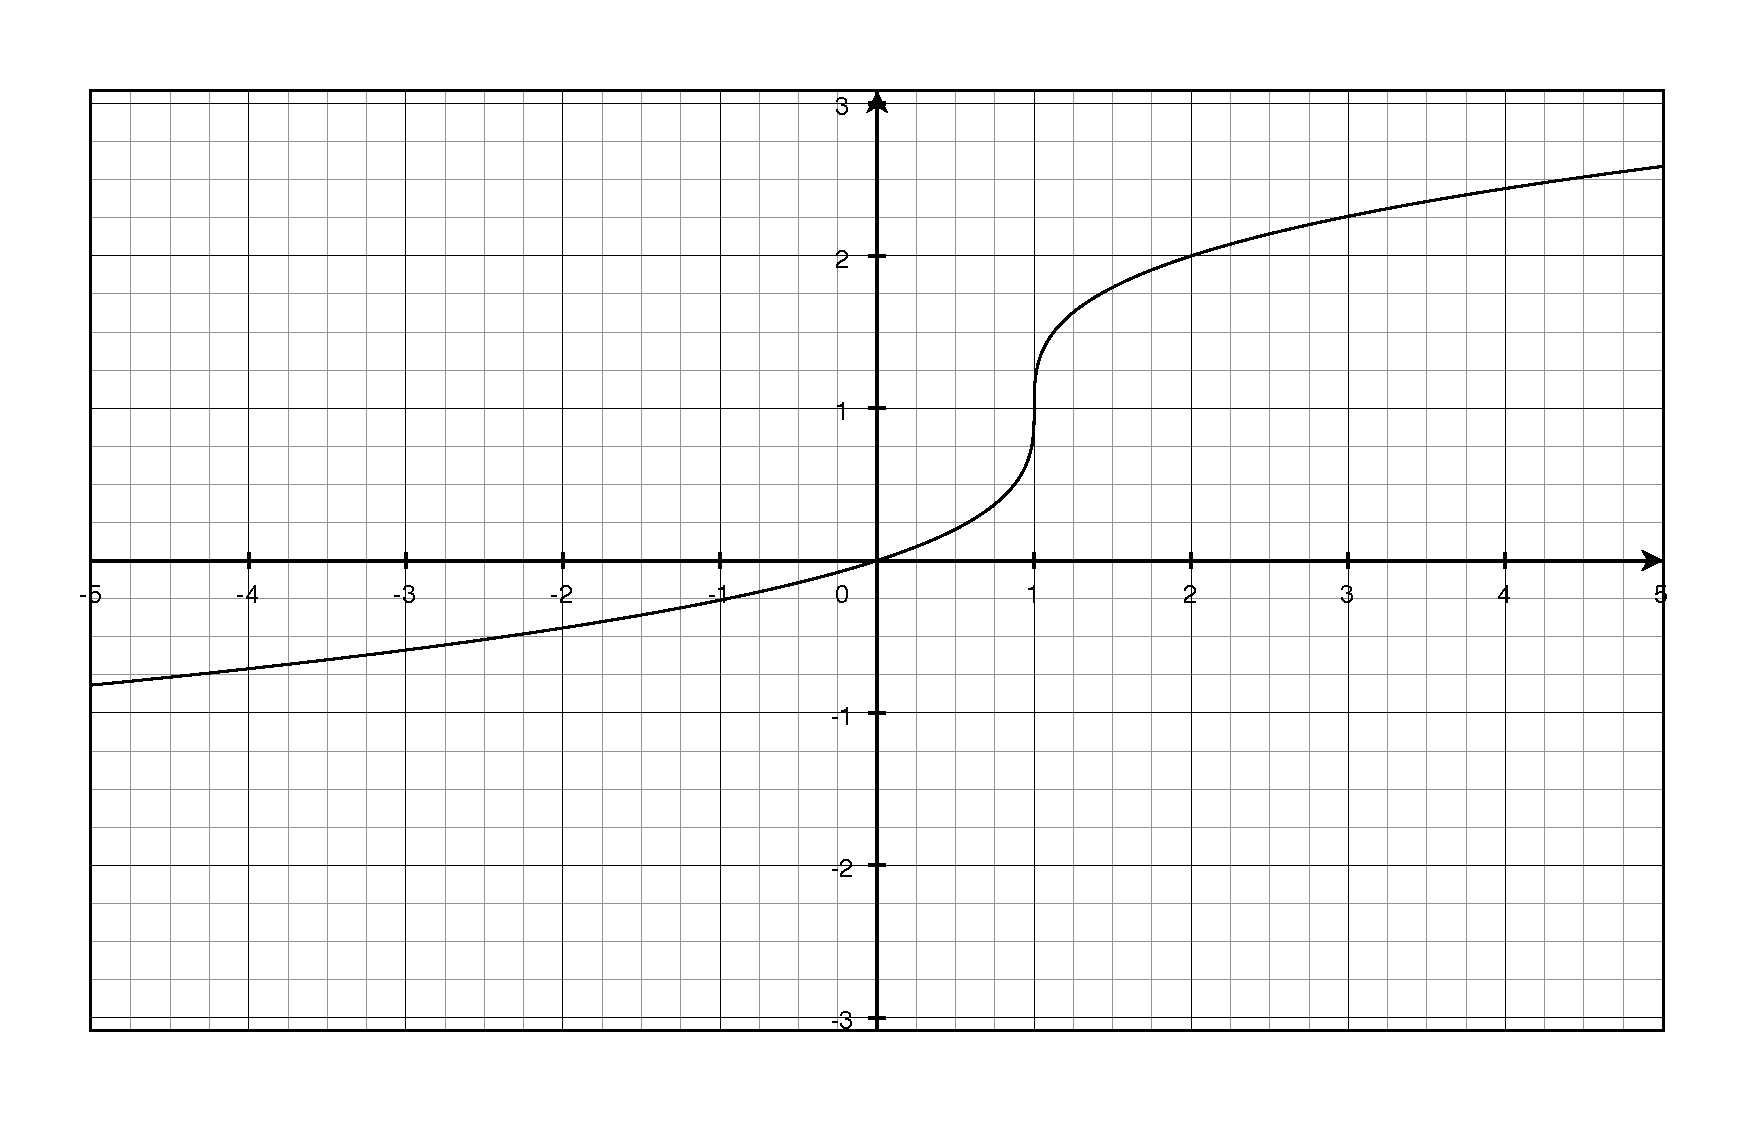
\includegraphics[scale=.3]{question7.eps}
%   \caption*{question 7}
% \end{figure}

% \begin{tabular}{cc}
%   \toprule
%   period & amplitude \\
%     $\pi$ & $2$ \\
%   \bottomrule
% \end{tabular}

\printanswers
\excludecomment{comment}

\ifprintanswers 
  \usepackage{2in1, lscape} 
\fi

\author{}
\date{\today}
\title{Math 142 \\ Homework Six}

\begin{document}

  \maketitle

  \section{Homework}
  Section 6.1: 

  \section{Extra Credit}
  TO DO

  \ifprintanswers

    \pagebreak

    \section{Section 6.1}
    \begin{description}
      \item[1] 
        \[
          72 \degree \cdot \frac{2 \pi}{360 \degree} = \boxed{ \frac{2 \pi}{5} }
        \]

      \item[2] 
        \[
          54 \degree \cdot \frac{2 \pi}{360 \degree} = \boxed{ \frac{3 \pi}{10} }
        \]

      \item[3] 
        \[
          -45 \degree \cdot \frac{2 \pi}{360 \degree} = \boxed{ -\frac{\pi}{4} }
        \]

      \item[4] 
        \[
          -60 \degree \cdot \frac{2 \pi}{360 \degree} = \boxed{ -\frac{\pi}{3} }
        \]

      \item[5] 
        \[
          -75 \degree \cdot \frac{2 \pi}{360 \degree} = \boxed{ -\frac{5 \pi}{12} }
        \]

      \item[13] 
        \[
          \frac{7 \pi}{6} \cdot \frac{360 \degree}{2 \pi} = \boxed{ 210 \degree }
        \]

      \item[14] 
        \[
          \frac{11 \pi}{3} \cdot \frac{360 \degree}{2 \pi} = \boxed{ 660 \degree }
        \]

      \item[15] 
        \[
          - \frac{5 \pi}{4} \cdot \frac{360 \degree}{2 \pi} = \boxed{ -225 \degree }
        \]

      \item[16] 
        \[
          - \frac{3 \pi}{2} \cdot \frac{360 \degree}{2 \pi} = \boxed{ -270 \degree }
        \]

      \item[17] 
        \[
          3 \cdot \frac{360 \degree}{2 \pi} \approx \boxed{ 172 \degree }
        \]

      \item[25] 
        \begin{align*}
          50 \degree + 360 \degree & = \boxed{ 410 \degree }
          50 \degree + 720 \degree & = \boxed{ 770 \degree }
          50 \degree - 360 \degree & = \boxed{ -310 \degree }
          50 \degree - 720 \degree & = \boxed{ -670 \degree }
        \end{align*}

      \item[26] 
        \begin{align*}
          135 \degree + 360 \degree & = \boxed{ 495 \degree }
          135 \degree + 720 \degree & = \boxed{ 855 \degree }
          135 \degree - 360 \degree & = \boxed{ -225 \degree }
          135 \degree - 720 \degree & = \boxed{ -585 \degree }
        \end{align*}

      \item[27] 
        \begin{align*}
          \frac{3 \pi}{4} + 2 \pi & = \boxed{ \frac{11 \pi}{4} }
          \frac{3 \pi}{4} + 4 \pi & = \boxed{ \frac{19 \pi}{4} }
          \frac{3 \pi}{4} - 2 \pi & = \boxed{ - \frac{5 \pi}{4} }
          \frac{3 \pi}{4} - 4 \pi & = \boxed{ - \frac{13 \pi}{4} }
        \end{align*}

      \item[28] 
        \begin{align*}
          \frac{11 \pi}{4} + 2 \pi & = \boxed{ \frac{19 \pi}{4} }
          \frac{11 \pi}{4} + 4 \pi & = \boxed{ \frac{27 \pi}{4} }
          \frac{11 \pi}{4} - 4 \pi & = \boxed{ - \frac{5 \pi}{4} }
          \frac{11 \pi}{4} - 6 \pi & = \boxed{ - \frac{13 \pi}{4} }
        \end{align*}

      \item[31] $430 \degree = 70 \degree + 360 \degree$
        The angles are \fbox{ coterminal }.

      \item[32] $330 \degree = 360 \degree - 30 \degree$
        The angles are \fbox{ coterminal }.

      \item[33] $\frac{17 \pi}{6} = \frac{5 \pi}{6} + 2 \pi$
        The angles are \fbox{ coterminal }.

      \item[34] The angles are \fbox{ not coterminal }.

      \item[35] $875 \degree = 155 \degree + 720 \degree$
        The angles are \fbox{ coterminal }.

      \item[36] The angles are \fbox{ not coterminal }.

      \item[37] $733 \degree - 720 \degree = \boxed{ 13 \degree }$

      \item[38] $361 \degree - 360 \degree = \boxed{ 1 \degree }$

      \item[39] $1110 \degree - 1080 \degree = \boxed{ 30 \degree }$

      \item[40] $-100 \degree + 360 \degree = \boxed{ 260 \degree }$

      \item[41] $-800 \degree + 1080 \degree = \boxed{ 280 \degree }$

      \item[42] $1270 \degree - 1080 \degree = \boxed{ 190 \degree }$

      \item[43] $\frac{17 \pi}{6} - 2 \pi = \frac{5 \pi}{6}$

      \item[44] $- \frac{7 \pi}{3} + 4 \pi = \frac{5 \pi}{3}$

      \item[45] $87 \pi - 86 \pi = \pi$

      \item[46] $10 - 2 \pi \approx 3.7168$

      \item[47] $\frac{17 \pi}{4} - 4 \pi = \frac{\pi}{4}$

      \item[48] $\frac{51 \pi}{2} - 25 \pi = \frac{\pi}{2}$

    \end{description}

  \else
    \vspace{1 cm}
    \begin{quote}
      \begin{em}
        TO DO
      \end{em}
    \end{quote}
    \hspace{1 cm} --Shunryu Suzuki
  \fi

\end{document}

